\documentclass[a4paper,12pt]{article}
\usepackage[utf8]{inputenc}
\usepackage{amsmath}
\usepackage{amssymb}
\usepackage{comment}
\usepackage{graphicx}
\usepackage[left=1cm, right=1cm, top=2cm, bottom=2cm]{geometry}
\title{\textbf{COM 5120 Communication Theory}}
\author{\textbf{Midterm Make-up Exam Answer}}
\date{November 17, 2022\\
15:30 $\sim$ 17:20
}
\begin{document}
    \maketitle
    \begin{enumerate}
        \item (13\%) 
            The answer is \textbf{(c)}, recall the definition of \textbf{sufficient statistic}, option (c) only contains $r_1$ and $r_2$ clearly not satisfied the definition.
            \begin{flushright}
                $\blacksquare$
            \end{flushright}
        %%%%%%%%%%%%%%%%%%%%%%%%%%%%%%%%%%%%%%%%%%%%%%
        \item (15\%) 
            \begin{align*}
                P_r\{x[n], \ n=1,2,\cdots,N|p\}=p^{\sum x[n]}(1-p)^{N-\sum x[n]}
            \end{align*}
            Denote $\overline{X}=\frac{1}{N}\sum\limits_{n=1}^Nx[n]$,
            \begin{align*}
                P_r\{ x[n],n=1,2,\cdots,N|p\}=p^{N\overline{X}}(1-p)^{N-N\overline{X}}
            \end{align*}
            To find 
            \begin{align*}
                \max_{p} P_r\{x[n],n=1,2,\cdots,N|p\}\\
                \frac{d\ln P_r\{ x[n],n=1,2,\cdots,N|p\}}{dp}=\cdots\\
                =\frac{N\overline{X}}{p}+\frac{N-N\overline{X}}{1-p}(-1)=0
            \end{align*}
            obtain $\widehat{p}=\overline{X}=\frac{1}{N}\sum\limits_{n=1}^{N}x[n]$.
            \begin{flushright}
                $\blacksquare$
            \end{flushright}
        %%%%%%%%%%%%%%%%%%%%%%%%%%%%%%%%%%%%%%%%%%%%%%
        \item (15\%) \\
        (a) \ $S_{\widehat{X}}(f)=|-j\text{sgn}(f)|^2S_X(f)=S_X(f)$, hence $R_{\widehat{X}}(\tau)=R_X(\tau)$\\
        (b) \ $S_{X\widehat{X}}(f)=S_X(f)(-j\text{sgn}(f))^*=j\text{sgn}(f)S_X(f)$, therefore, $R_{X\widehat{X}}(\tau)=-R_{X}(\tau)$\\
        (c) \ $R_Z(\tau)=E\left[ \left( X(t+\tau)+j\widehat{X}(t+\tau)\right)\left( X(t)-j\widehat{X}(t)\right)\right]$, expanding we have
        \begin{align*}
            R_Z(\tau)=R_X(\tau)+R_{\widehat{X}}(\tau)-j\left[ R_{X\widehat{X}}(\tau)-R_{\widehat{X}X}(\tau)\right]
        \end{align*}
        Using $R_{\widehat{X}}(\tau)=R_X(\tau)$, and the fact that $R_{X\widehat{X}}(\tau)=-\widehat{R}_X(\tau)$ is an odd function (since it is the HT of an even signal) we have $R_{\widehat{X}X}(\tau)=R_{X\widehat{X}}(-\tau)=-R_{X\widehat{X}}(\tau)$, we have 
        \begin{align*}
            R_Z(\tau)=2R_X(\tau)-jR_{X\widehat{X}}(\tau)=2R_X(\tau)+j2\widehat{R}_X(\tau)
        \end{align*}
        Taking FT of both sides we have
        \begin{align*}
            S_Z(f)=2S_X(f)+j2(-j\text{sgn}(f)S_X(f))=2(1+\text{sgn}(f))S_X(f)=4S_X(f)u_{-1}(f)
        \end{align*}\\
        % (d) \ We have
        % \begin{align*}
        %     R_{X_l}(t+\tau,t)&=E\left[ Z(t+\tau)e^{-j2\pi f_0(t+\tau)}Z^*(t)e^{j2\pi f_0t}\right]\\
        %     &=e^{-j2\pi f_0\tau}R_z(\tau)
        % \end{align*}
        % This shows that $X_l(t)$ is WSS. Taking FT, we have $S_{X_l}(f)=S_Z(f-f_0)=4S_X(f-f_0)u_{-1}(f-f_0)$, this shows that $X_l(t)$ is lowpass. Also from above $R_X(\tau)=\frac{1}{2}\text{Re}[R_Z(t)]=\frac{1}{2}\text{Re}[R_{X_l}(\tau)e^{-j2\pi f_0\tau}]$. This shows that $R_{X_l}(\tau) $ is twice the LP equivalent of $R_X(\tau)$.
        %     \begin{flushright}
        %         $\blacksquare$
        %     \end{flushright}
        %%%%%%%%%%%%%%%%%%%%%%%%%%%%%%%%%%%%%%%%%%%%%%
        \item (14\%) \\
        (a)\ To show that the waveforms $f_n(t),\ n=1, 2, 3$ are orthogonal we have to prove that: \\
        \begin{align*}
            \int_{-\infty}^{\infty} f_m(t)f_n(t)\, dt=0, \qquad m\neq n
        \end{align*}
        \begin{figure}[h]
        	\centering
        	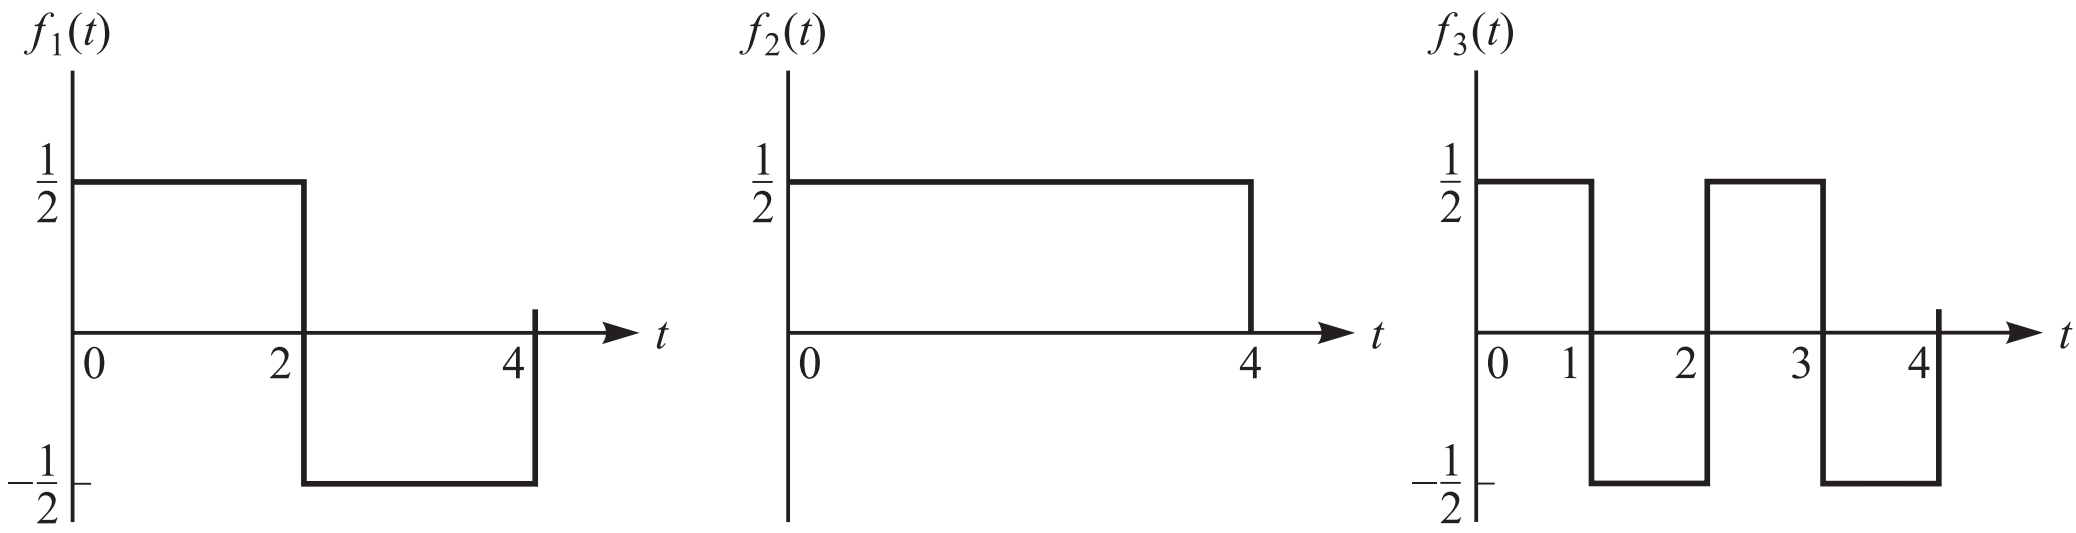
\includegraphics[scale=0.3]{Mid_fig1.png}
        	\caption{three waveforms $f_1(t)$, $f_2(t)$, $f_3(t)$}
        % 	\label{fig}
        \end{figure} \\
        Clearly: 
        \begin{align*}
            c_{12} &= \int_{-\infty}^{\infty}f_1(t)f_2(t)\, dt=\int_{0}^{4}f_1(t)f_2(t)\, dt = \int_{0}^{2}f_1(t)f_2(t)\, dt+\int_{2}^{4}f_1(t)f_2(t)\, dt \\
            &= \int_{0}^{2}\frac{1}{2} \cdot \frac{1}{2}\, dt + \int_{2}^{4}\frac{-1}{2} \cdot \frac{1}{2}\, dt = \frac{1}{4}\int_{0}^{2}1\, dt-\frac{1}{4}\int_{2}^{4}1\, dt \\
            &= \frac{1}{4} \cdot 2-\frac{1}{4} \cdot (4-2) = 0 
        \end{align*}
        Similarly: 
        \begin{align*}
            c_{13} &= \int_{-\infty}^{\infty}f_1(t)f_3(t)\,dt = \int_{0}^{4}f_1(t)f_3(t)\, dt \\
            &= \int_{0}^{1}f_1(t)f_3(t)\, dt + \int_{1}^{2}f_1(t)f_3(t)\, dt + \int_{2}^{3}f_1(t)f_3(t)\, dt + \int_{3}^{4}f_1(t)f_3(t)\, dt \\
            &= \int_{0}^{1}\frac{1}{2} \cdot \frac{1}{2}\, dt + \int_{1}^{2}\frac{1}{2} \cdot \frac{-1}{2}\, dt + \int_{2}^{3}\frac{-1}{2} \cdot \frac{1}{2}\, dt + \int_{3}^{4}\frac{-1}{2} \cdot \frac{-1}{2}\, dt \\ 
            &=\frac{1}{4}\int_{0}^{1}1\, dt-\frac{1}{4}\int_{1}^{2}1\, dt-\frac{1}{4}\int_{2}^{3}1\, dt+\frac{1}{4}\int_{3}^{4}1\, dt=0
        \end{align*}
        and: 
        \begin{align*}
            c_{23} &= \int_{-\infty}^{\infty}f_2(t)f_3(t)\,dt=\int_{0}^{4}f_2(t)f_3(t)\, dt \\
            &= \int_{0}^{1}f_2(t)f_3(t)\, dt + \int_{1}^{2}f_2(t)f_3(t)\, dt + \int_{2}^{3}f_2(t)f_3(t)\, dt + \int_{3}^{4}f_2(t)f_3(t)\, dt \\
            &= \int_{0}^{1}\frac{1}{2} \cdot \frac{1}{2}\, dt + \int_{1}^{2}\frac{1}{2} \cdot \frac{-1}{2}\, dt + \int_{2}^{3}\frac{1}{2} \cdot \frac{1}{2}\, dt + \int_{3}^{4}\frac{1}{2} \cdot \frac{-1}{2}\, dt \\ 
            &= \frac{1}{4}\int_{0}^{1}1\, dt-\frac{1}{4}\int_{1}^{2}1\, dt 
             + \frac{1}{4}\int_{2}^{3}1\, dt-\frac{1}{4}\int_{3}^{4}1\, dt = 0
        \end{align*}
        Thus, the signals $f_n(t)$ are orthogonal. It is also straightforward to prove that the signals have unit energy:
        \begin{align*}
            \int_{-\infty}^{\infty} |f_i(t)|^2\, dt=1,\ i=1,2,3. 
        \end{align*}
        Hence, they are orthonormal.\\ \\ 
        (b) We first determine the weighting coefficients
        \begin{align*}
            x_n=\int_{-\infty}^{\infty}x(t)f_n(t)\, dt,\ n=1,2,3, \;\;\; \text{where} \; x = \left\{ 
            \begin{aligned}
                -2, \; 0 \leq t < 1 \\
                 6, \; 1 \leq t < 3 \\ 
                 4, \; 3 \leq t < 4 \\
            \end{aligned}
            \right.
        \end{align*}
        \begin{align*}
            x_1 &= \int_{0}^{4}x(t)f_1(t)\, dt \\
                &= \int_{0}^{1}x(t)f_1(t)\, dt + \int_{1}^{2}x(t)f_1(t)\, dt 
                 + \int_{2}^{3}x(t)f_1(t)\, dt + \int_{3}^{4}x(t)f_1(t)\, dt \\
                &= \int_{0}^{1} -2 \cdot \frac{1}{2}\,dt + \int_{1}^{2} 6 \cdot \frac{1}{2}\,dt 
                 + \int_{2}^{3} 6 \cdot \frac{-1}{2}\,dt + \int_{3}^{4} 4 \cdot \frac{-1}{2}\,dt \\
                &= -1 \int_{0}^{1}1 \; dt + 3 \int_{1}^{2}1 \; dt 
                 - 3 \int_{2}^{3}1 \; dt - 2 \int_{3}^{4}1 \; dt = -3 \\
            x_2 &= \int_{0}^{4}x(t)f_2(t)\, dt \\
                &= \int_{0}^{1}x(t)f_2(t)\, dt + \int_{1}^{2}x(t)f_2(t)\, dt 
                 + \int_{2}^{3}x(t)f_2(t)\, dt + \int_{3}^{4}x(t)f_2(t)\, dt \\
                &= \int_{0}^{1} -2 \cdot \frac{1}{2}\,dt + \int_{1}^{2} 6 \cdot \frac{1}{2}\,dt 
                 + \int_{2}^{3} 6 \cdot \frac{1}{2}\,dt + \int_{3}^{4} 4 \cdot \frac{1}{2}\,dt \\
                &= -1 + 3 + 3 + 2 = 7 \\
            x_3 &= \int_{0}^{4}x(t)f_3(t)\, dt \\
                &= \int_{0}^{1}x(t)f_3(t)\, dt + \int_{1}^{2}x(t)f_3(t)\, dt 
                 + \int_{2}^{3}x(t)f_3(t)\, dt + \int_{3}^{4}x(t)f_3(t)\, dt \\
                &= \int_{0}^{1} -2 \cdot \frac{1}{2}\,dt + \int_{1}^{2} 6 \cdot \frac{-1}{2}\,dt 
                 + \int_{2}^{3} 6 \cdot \frac{1}{2}\,dt + \int_{3}^{4} 4 \cdot \frac{-1}{2}\,dt \\
                &= -3
        \end{align*}
        As it is observed, $x(t)$ is orthogonal to the signal waveforms $f_n(t),\ n=1,2,3$ and thus it can not represented as a linear combination of these funtions.
            \begin{flushright}
                $\blacksquare$
            \end{flushright}
        %%%%%%%%%%%%%%%%%%%%%%%%%%%%%%%%%%%%%%%%%%%%%%
        \item (14\%) \\
        (a) \ Consider the QAM constellation of Figure 2. Using the Pythagorean theorem we can find the radius of the inner circle as:
        \begin{align*}
            a^2+a^2=A^2\Longrightarrow a=\frac{1}{\sqrt{2}}A
        \end{align*}
        The radius of the outer circle an be found using the cosine rule. Since $b$ is the third side of a triangle with $a$ and $A$ the two other sides and angle between then equal to $\theta=105^\circ$, we obtain:
        \begin{align*}
            b^2=a^2+A^2-2aA\cos105^\circ\Longrightarrow b=\frac{1+\sqrt{3}}{2}A
        \end{align*}\\
        (b) \ If we denote by $r$ the radius of the circle, then using the cosine theorem we obtain:
        \begin{align*}
            A^2=r^2+r^2-2r\cos 45^\circ\Longrightarrow r=\frac{A}{\sqrt{2-\sqrt{2}}}
        \end{align*}
            \begin{flushright}
                $\blacksquare$
            \end{flushright}
        %%%%%%%%%%%%%%%%%%%%%%%%%%%%%%%%%%%%%%%%%%%%%%
        \item (14\%) \\ 
            (a) The correlation type demodulator employes a filter: \\ 
            $$f(t) = \left\{ 
            \begin{aligned}
                \frac{1}{\sqrt{T}}, \; 0 \leq t < T \\
                 0, \; otherwise \\ 
            \end{aligned}
            \right.
            $$ \\ 
            Hence, the sampled outputs of the crosscorrelators are: \\
            $$r = s_m + n, \; m = 0, 1$$ \\ 
            where $s_0 = 0, \; s_1 = A\sqrt{T}$ and the noise term $n$ is a zero-mean Gaussian random variable with variance:
            $$\sigma_n^2 = \frac{N_0}{2}$$ \\ 
            The probability density function for the sampled output is: \\
            \begin{align*}
                p(r|s_0) &= \frac{1}{\sqrt{\pi N_0}}e^{-\frac{r^2}{N_0}} \\ 
                p(r|s_1) &= \frac{1}{\sqrt{\pi N_0}}e^{-\frac{(r - A\sqrt{T})^2}{N_0}}
            \end{align*}
            Since the signals are equally probable, the optimal detector decides in favor of $s_0$ if 
            \begin{align*}
                PM(\bf r| \bf s_0) &= p(r|s_0) > p(r|s_1) = PM(\bf r| \bf s_1) \\
            \end{align*}
            otherwise it decides in favor of $s_1$. The decision rule may be expressed as:
            \begin{figure}[h]
            	\centering
            	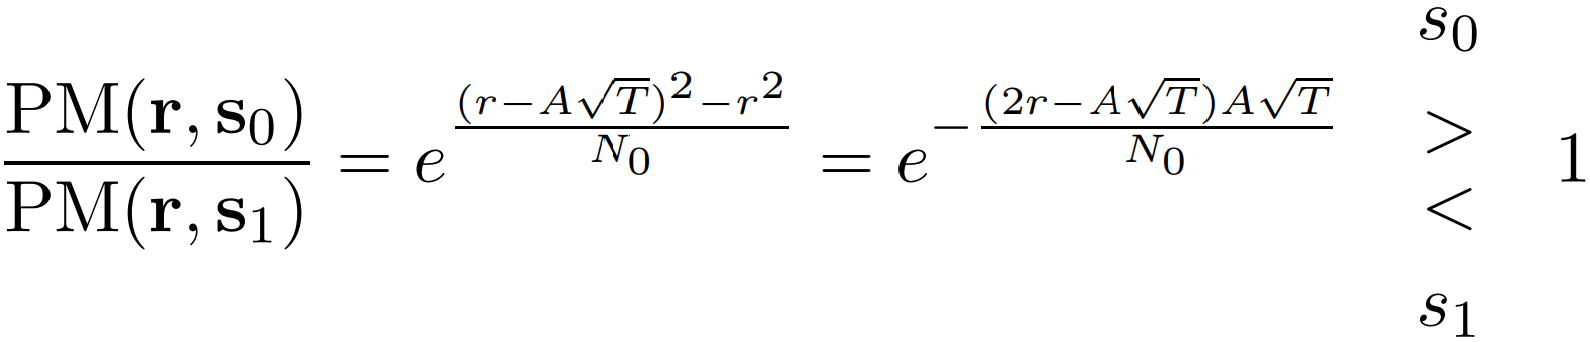
\includegraphics[scale=0.3]{Mid_math1.png}
            \end{figure}
            \newpage
            or equivalently: \\ 
            \begin{figure}[h]
            	\centering
            	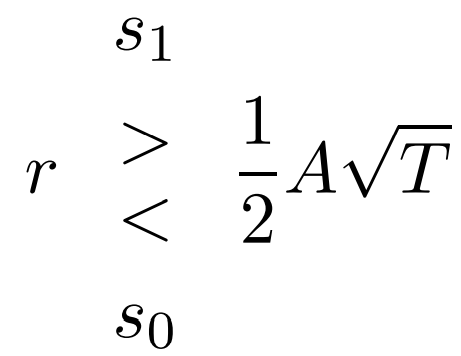
\includegraphics[scale=0.3]{Mid_math2.png}
            \end{figure} \\
            The optimum threshold is $\frac{1}{2}A\sqrt{T}$. \\ \\
            (b) The average probability of error is: \\
            \begin{align*}
                P(e) &= \frac{1}{2}P(e|s_0) + \frac{1}{2}P(e|s_1) \\
                     &= \frac{1}{2}\int_{\frac{1}{2}A\sqrt{T}}^{\infty}p(r|s_0)dr 
                      + \frac{1}{2}\int_{-\infty}^{\frac{1}{2}A\sqrt{T}}p(r|s_0)dr \\
                     &= \frac{1}{2}\int_{\frac{1}{2}A\sqrt{T}}^{\infty}\frac{1}{\sqrt{\pi N_0}}e^{-\frac{r^2}{N_0}}dr + \frac{1}{2}\int_{-\infty}^{\frac{1}{2}A\sqrt{T}}\frac{1}{\sqrt{\pi N_0}}e^{-\frac{(r - A\sqrt{T})^2}{N_0}}dr \\ 
                     &= \frac{1}{2}\int_{\frac{1}{2}\sqrt{\frac{2}{N_0}}A\sqrt{T}}^{\infty}\frac{1}{\sqrt{2\pi}}e^{-\frac{x^2}{2}}dx + \frac{1}{2}\int_{-\infty}^{-\frac{1}{2}\sqrt{\frac{2}{N_0}}A\sqrt{T}}\frac{1}{\sqrt{2\pi}}e^{-\frac{x^2}{2}}dx \\
                     &= Q[\frac{1}{2}\sqrt{\frac{2}{N_0}}A\sqrt{T}] = Q[\sqrt{\text{SNR}}], \text{where} \;\; \text{SNR} = \frac{\frac{1}{2}A^2T}{N_0} \\
                    %  \intertext{Thus, the on-off signaling requires a factor of two more energy to achieve the same probability of error as the antipodal signaling.}
            \end{align*} \\
            Thus, the on-off signaling requires a factor of two more energy to achieve the same probability of error as the antipodal signaling.
            \begin{flushright}
                $\blacksquare$
            \end{flushright}
        %%%%%%%%%%%%%%%%%%%%%%%%%%%%%%%%%%%%%%%%%%%%%%
        \item (15\%) 
            The PDF of the noise $n$ is: 
            \begin{align*}
                p(n) = \frac{1}{\sqrt{2\sigma}}e^{-|n|\sqrt{\frac{2}{\sigma}}} = \frac{\lambda}{2}e^{-\lambda|n|} \text{, where} \;\; \lambda = \sqrt{\frac{2}{\sigma}}
            \end{align*}
            % \newpage
            The optimal receiver uses the criterion: 
            \begin{figure}[h]
                \centering
                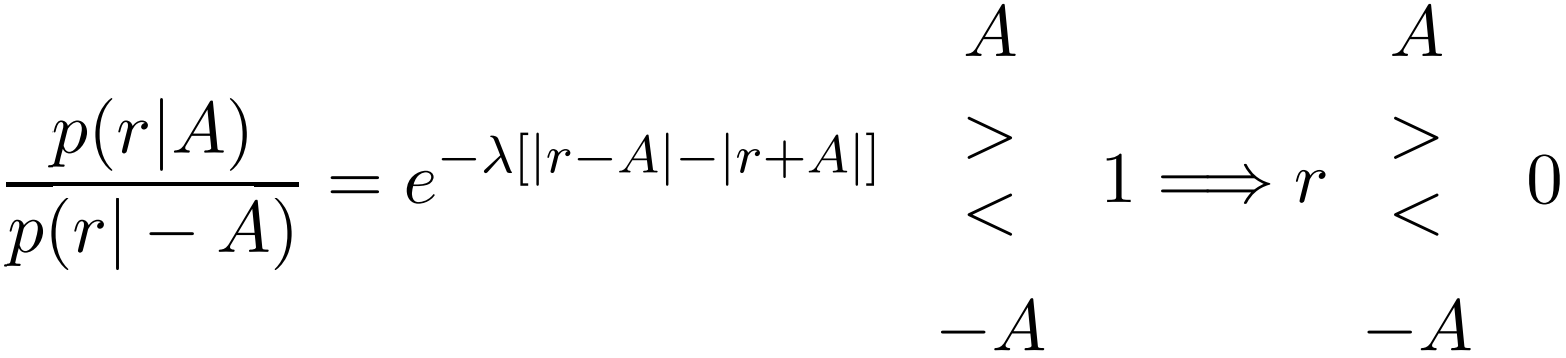
\includegraphics[scale=0.3]{Mid_math3.png}
                % \caption{Caption}
                % \label{fig:my_label}
            \end{figure}
            \newpage
            The average probability of error is: \\
            \begin{align*}
                P(e) &= \frac{1}{2}P(e|A) + \frac{1}{2}P(e|-A) \\
                     &= \frac{1}{2}\int_{-\infty}^{0}f(r|A)dr 
                      + \frac{1}{2}\int_{0}^{\infty}f(r|-A)dr \\
                     &= \frac{1}{2}\int_{-\infty}^{0}\frac{\lambda}{2}e^{-\lambda|r - A|}dr 
                      + \frac{1}{2}\int_{0}^{\infty}\frac{\lambda}{2}e^{-\lambda|r + A|}dr \\
                     &= \frac{\lambda}{4}\int_{-\infty}^{A}e^{-\lambda|x|}dx 
                      + \frac{\lambda}{4}\int_{A}^{\infty}e^{-\lambda|x|}dx \\ 
                     &= 2 \cdot \frac{\lambda}{4}\int_{A}^{\infty}e^{-\lambda|x|}dx \\ 
                     &= \frac{\lambda}{2} \cdot \frac{-1}{\lambda} \cdot (e^{-\lambda \infty} - e^{-\lambda A}) = \frac{-1}{2} \cdot (0 - e^{-\lambda A}) \\
                     &= \frac{1}{2}e^{-\lambda A} = \frac{1}{2}e^{-\sqrt{\frac{2}{\sigma}}A}
            \end{align*}
            \begin{flushright}
                $\blacksquare$
            \end{flushright}
        %%%%%%%%%%%%%%%%%%%%%%%%%%%%%%%%%%%%%%%%%%%%%%
    \end{enumerate}
    \rule{\textwidth}{0.4pt}
\end{document}
